\chapter{Overview of traditional GSM networks}

\section{What is GSM?}
GSM, or Global System for Mobile Communications,  is a European standard for 
the Mobile telecommunications and it is considered as one of the most popular
standard worldwide.There are thirteen different frequency bands defined in GSM.
However, the 850 MHz, 900 MHz, 1800 MHz, and 1900 MHz bands are the most 
commonly used. The frequency bands employed within each of the four ranges are 
similarly organized. They differ essentially only in the frequencies, such that 
various synergy effects can be taken advantage of; hence, here we give some 
details only for the usage in the 900 MHz band.


In the 900 MHz band, a total of 70 MHz bandwidth is allocated, two 25-MHz 
frequency bands for uplink and downlink and a 20 MHz unused guard band between 
them. The MS transmits in the 890 to 915 MHz range (uplink) and the BTS 
transmits in the 935 to 960 MHz (downlink) band. This corresponds to 124 duplex
channels, where each channel within a BTS is referred to as an Absolute Radio 
Frequency Channel Number (ARFCN). This number describes a pair of frequencies, 
one uplink and one downlink, and is given a channel index between C0 and C123, 
with C0 designated as the beacon channel. An ARFCN could be used to calculate 
the exact frequency (in MHz) of the radio channel. In the GSM 900 band, this is 
computed by the following equations:

\begin{align}
F_{uplink}(n) &= 890 + 0.2*n \qquad & 1\leq{}n\leq{}124 \nonumber\\
F_{downlink}(n) &= F_{uplink}(n) + 45  \qquad & 1\leq{}n\leq{}124 \nonumber
\end{align}

Similar formulae are also defined for the other GSM frequency bands.


The principle component groups of a GSM network are as follows:
\begin{itemize}
	\item The Mobile Station (MS)
	\item The Base Station System (BSS)
	\item The Network Switching System(NSS)
\end{itemize}


\begin{figure}[h]
\centering
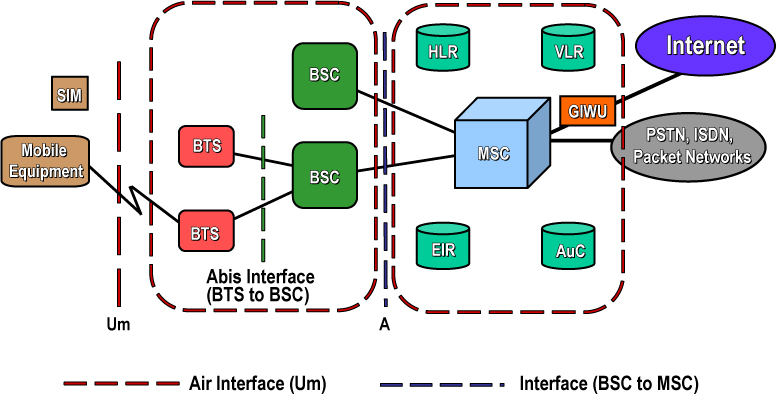
\includegraphics[width=1\textwidth]{gsmArch}
\caption[The conventional GSM architecture]{The conventional GSM architecture. \emph{Source: \url{http://www.hill2dot0.com/wiki/index.php?title=Image:G2407\_{}GSM-Architecture.jpg} [Accessed on Oct 22, 2013]}}
\label{gsmArch}
\end{figure}

\subsection{Mobile Station}
The MS consists of two parts, the Mobile Equipment (ME) and  Subscriber 
Identity module (SIM). The ME has an identity number called the International
 Mobile Equipment Identity (IMEI) associated with it, which is unique for 
that particular device and permanently stored in it.The SIM card consists 
the International Mobile Subscriber Identity(IMSI) number which is used 
to identify the subscriber to the system. The IMEI and the IMSI are independent 
of each other and hence allow personal mobility.

\subsection{Base Station System}
The GSM Base Station System is the equipment located at a cell site. It
comprises of a combination of digital and RF equipment. The BSS provides 
the link between the MS and the Mobile Services Switching Centre (MSC).
The BSS consists mainly of:
\begin{description}
	\item[The Base Transceiver Station(BTS)]  
	The BTS contains the RF components that provide the air interface for
 a particular cell. This is the part of the GSM network which communicates
 with the MS. The antenna is included as part of the BTS.
	\item[The Base Station Controller(BSC)]  
	The BSC  provides the control for the BSS. The BSC communicates directly 
with the MSC. The BSC may control single or multiple BTSs. Crucial functions 
like radio channel link establishment, frequency hopping, and handovers from
one cell to another.

\end{description}

\subsection{Network Switching Subsystem}
The Network Switching Subsystem includes 
the main switching functions of the GSM network. It also contains the databases
required for subscriber data and mobility management. Its main function is 
to manage communications between the GSM network and other telecommunications 
networks. The main components of the Network Switching System are: 

	
\subsubsection*{Mobile Services Switching Centre(MSC)}
The MSC does call-switching 
and its overall purpose is the same as that of any telephone exchange. When 
the MSC provides the interface between the PSTN and the BSSs in the GSM 
network it will be known as a Gateway MSC. In this position it will provide 
the switching required for all MS originated or terminated traffic. Each 
MSC provides service to MSs located within a defined geographic coverage 
area. One MSC is capable of supporting a regional capital with approximately
 one million inhabitants. 
The functions carried out by the MSC are: Call Processing, Operations and 
Maintenance Support, Internetwork Interworking and Billing

\subsubsection*{Home Location Register (HLR)}
The HLR is a central database that contains the details of each mobile phone 
subscriber that is authorized to use the GSM core network. The IMSI of 
each SIM acts as a primary key to each HLR record. Each MSISDN is
also a primary key to the HLR record. The HLR data is stored 
as long as a subscriber remains with the mobile phone operator.
Data stored in the HLR against each IMSI are, GSM services that the 
subscriber has requested, GPRS settings to allow the subscriber to 
access packet services, current location of the subscriber, etc.

\subsubsection*{Visitor Location Register (VLR)}
The VLR is a database of the subscribers who have roamed into the jurisdiction
of the MSC which it serves. Each main base station in the network is served by 
exactly one VLR, hence a subscriber cannot be present in more than
one VLR at a time.The data stored in the VLR has either been received
from the HLR, or collected from the MS. Data stored includes: IMSI
(the subscriber's identity number), authentication data, MSISDN, 
GSM services that the subscriber is allowed to access, the HLR address 
of the subscriber.



\section{Um Interface}
The Um interface is the air interface of the GSM mobile telephone standard. 
It is the interface between the MS and the BTS. It is called Um because it 
is the mobile analog to the U interface of ISDN. Um is defined in the 
GSM 04.xx and 05.xx series of specifications.


The layers of GSM are initially defined in GSM 04.01 Section 7 and roughly 
follow the OSI model. Um is defined in the lower three layers of the model.

\subsection{Physical Layer (L1)}
The Um physical layer is defined in the GSM 05.xx series of specifications,
 with the introduction and overview in GSM 05.01. For most channels,
Um L1 transmits and receives 184-bit control frames or 260-bit vocoder 
frames over the radio interface in 148-bit bursts with one burst per 
timeslot. There are three sublayers:

\subsubsection*{Radiomodem}
 
This is the actual radio transceiver. GSM uses 8PSK modulation with 1 bit per
symbol which produces a 13/48 MHz (270.833 kHz or 270.833 K symbols/second)
symbol rate and a channel spacing of 200 kHz. Since adjacent channels overlap, 
the standard does not allow adjacent channels to be used in the same cell. The 
standard defines several bands ranging from 400 MHz to 1990 MHz.GSM is frequency
 duplexed, meaning that the network and MS transmit on different frequencies, 
allowing the BTS to transmit and receive at the same time. Transmission from 
the network to the MS is called the ``downlink" and that from the MS to the network 
is called the ``uplink". The GSM uplink and downlink bands are separated by 45 or 
50 MHz. Uplink/downlink channel pairs are identified by an index called the 
ARFCN. Within the BTS, these ARFCNs are given arbitrary carrier indexes 
C0..Cn-1, with C0 designated as a Beacon Channel and always operated at constant
 power. The radio channel is time-multiplexed into 8 timeslots, each with a 
duration of 156.25 symbol periods. These 8 timeslots form a frame of 1,250 
symbol periods. The capacity associated with a single timeslot on a single 
ARFCN is called a physical channel (PCH) and referred to as ``CnTm" where n is
a carrier index and m is a timeslot index (0-7).Each timeslot is occupied by 
a radio burst with a guard interval, two payload fields, tail bits, and a 
midamble.
	
	
\subsubsection*{Multiplexing and Timing}
GSM uses TDMA to subdivide each
radio channel into as many as 16 traffic channels or as many as 64 control 
channels. The multiplexing patterns are defined in GSM 05.02.Each physical
channel is time-multiplexed into multiple logical channels according to 
the rules of GSM 05.02. Traffic channel multiplexing follows a 26-frame
(0.12 second) cycle called a "multiframe". Control channels follow a 
51-frame multiframe cycle. The C0T0 physical channel carries the 
synchronization channel(SCH), which encodes the timing state of the 
BTS to facilitate synchronization to the TDMA pattern.
	
	
\subsubsection*{FEC Coding} The coding sublayer provides forward error 
correction. As a general rule, each GSM channel uses a block parity code
(usually a Fire code), a rate-1/2, 4th-order convolutional code and a 
4-burst or 8-burst interleaver.



\subsection{Data Link Layer(L2)}
The Um data link layer, LAPDm, is defined in GSM 04.05 and 04.06. 
LAPDm is the mobile analog to ISDN's LAPD.

\subsection{Network layer(L3)}
The Um network layer is defined in GSM 04.07 and 04.08 and has three sublayers.
A subscriber terminal must establish a connection in each sublayer before 
accessing the next higher sublayer.

\begin{description}
	\item[Radio Resource (RR)] This sublayer manages the assignment and 
release of logical channels on the radio.

	\item[Mobility Management (MM)] This sublayer authenticates users and 
tracks their movements from cell to cell. It is normally terminated in 
the VLR or HLR.

	\item[Call Control (CC)] This sublayer connects telephone calls and is 
taken directly from ITU-T Q.931. GSM 04.08 Annex E provides a table of 
corresponding paragraphs in GSM 04.08 and ITU-T Q.931 along with a summary
of differences between the two. The CC sublayer is terminated in the MSC.

\end{description}

The access order is RR, MM, CC. The release order is the reverse of that. 
Note that none of these sublayers terminate in the BTS itself. The standard 
GSM BTS operates only in layers 1 and 2.
